\documentclass[a4paper, 11pt]{jsarticle}
\usepackage{amsmath, amssymb}
\usepackage{bm}
\usepackage[dvipdfmx]{graphicx, color}
\usepackage{url}
\usepackage[at]{easylist}

\setlength{\topmargin}{-10.4truemm}
\setlength{\evensidemargin}{-5.4truemm}
\setlength{\oddsidemargin}{-5.4truemm}
\setlength{\headheight}{17pt}
\setlength{\headsep}{10mm}
\addtolength{\headsep}{-17pt}
\setlength{\footskip}{5mm}

\pagenumbering{arabic}

\title{様々な大きさのTravelling Salesman Problemに対する解法に関する研究}
\author{大阪府立大学工業高等専門学校 電子情報コース 3年 帖佐 克己}
\date{2014年2月26日}

\begin{document}
\maketitle
\thispagestyle{empty}
\pagebreak
\tableofcontents
\pagebreak

\section{用語説明}

この後に出てくる用語に関して、ここで事前に説明しておく。 \\

\begin{easylist}[itemize]

		@ 時間計算量 \\
			時間計算量とは、与えられた問題をとく際に要するステップ数を意味し、入力データの大きさ(ビット数などで表現できる)の関数として表される。例えば、ある問題に対する解法が$n$ビットの入力に対して、ある計算モデルで$n^2$ステップで動作する場合、時間計算量は$n^2$となる。また、今回の研究では、アルゴリズムの計算量を表す際に一般的に使われる$O$記法を用いて、$O(n^2)$と表す。 \\

		@ 選択 \\
			個体の適応度を基に、適応度の高い個体がより多くの子孫を残すように選択すること。本研究では以下の2つの手法を用いたのでここで詳しく説明する。
			@@ エリート選択 \\
				適応度の高い個体をそのまま次世代に複製する手法。この手法により、その辞典で最も良い解が交叉で壊されないという利点がある。一般的に他の手法を組み合わせて用いられる。
			@@ ルーレット選択 \\
				適応度に比例して、親として選択される確率を定めて、その確率に従ってランダムに選ぶという手法。個体数を$n$,ある個体$i$の適応度を$f_i$とすると、ある個体$i$が選択される確率$p_i$は以下のようになる。
				\begin{eqnarray*}
					p_i = \frac{f_i}{\displaystyle \sum_{j=1}^{n}f_j}
				\end{eqnarray*}

		@ 突然変異 \\
			各遺伝子に対して、一定確率で、変更を行う。突然変異は局所最適解に集団の遺伝子が収束してしまうのを防ぐ役割を果たす。本研究では、突然変異率を3\%とし、以下の手法を用いた。
			@@ 逆位 \\
				ランダムに選ばれた2点間の要素の順序を入れ替える手法。この手法は、遺伝子の要素を変更せずに順番のみを変更させるという特徴を持つ。 \\
\pagebreak

		@ 交叉 \\
			選択によって選出された個体に対して、ある交叉位置で双方の染色体の一部を取ってきて、子孫の染色体を作ること。本研究では以下の手法を用いたのでここで詳しく説明する。
			@@ 順序交叉 \\
				ランダムに切れ目を決定し、子1に対し、切れ目の左側では親1の遺伝子をそのまま受け継ぎ、右側では親1の遺伝子を親2の遺伝子の出現順序に並べ替えるという手法。この手法は、遺伝子の要素を変更せずに順番のみを変更させるという特徴を持つ。
				\begin{figure}[htbp]
					\begin{center}
						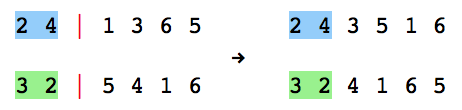
\includegraphics[width=10cm]{img/order_crossover.png}
						\caption{順序交叉}
						\label{crossover}
					\end{center}
				\end{figure}
	\end{easylist}

\pagebreak

	\section{Travelling Salesman Problemとは}

	Travelling Salesman Problem(巡回セールスマン,以下TSPと表記)とは都市の集合と各2都市間の移動コストが与えられたとき、すべての都市をちょうど一度ずつ巡り出発地に戻る順回路の総移動コストが最小のものを求める(セールスマンが所定の複数の都市を1回だけ巡回する場合の最短経路を求める)組み合わせ最適化問題である。
	問題の大きさは、都市の数で表される。また、この問題は計算複雑性理論においてNP-Hardと呼ばれる問題のクラスに属する。すなわち、問題の大きさに関する決定性を確かめるための多項式時間の計算量のアルゴリズムが見つかりそうにないと予想されている、計算量的に困難な問題である。 \newline

	今回の研究に関しては、三角不等式を満たし、都市を平面上の点、都市間の距離を平面上のユークリッド距離とする部分問題である平面TSPを扱う。

	\section{研究目的}

	人間の脳が普段当たり前のように行っていることをコンピュータに行わせようとすると、人間の脳のようにうまくいかないことが多々ある。TSPもその一例である。移動というのは人間が生活を送る上で不可欠な行為である。人間の脳は目的地が複数あったとしてもおおよそ最短コストである経路を導きだすことが出来る。それに対して、どれだけコンピュータが挑むことが出来るのかを様々なアプローチで確かめる。

	\section{研究方法}

	いくつかの座標データを用意し、いくつかのアプローチを実装したプログラムを実行し、比較する。
	今回は、bitを用いた動的計画法による解法と遺伝的アルゴリズムを用いた解法の2通りのアプローチを行う。

	\subsection{アプローチ1 bitを用いた動的計画法による解法}

	一般的なアプローチとして最初に思いつく方法が、取りうる経路をすべて列挙し、すべてのコストを確かめるというものがある。しかし頂点数を$n$とするとこれは時間計算量が$O(n \times n!)$がかかり、$n$が11程度で市販のPCでは時間がかかってしまい、解けないようになる。そこで、すでに行った場所と今いる場所がわかればそれ以前の情報は不要であることを利用して、bitですでに行った場所を管理し、 (今いる場所,すでに行った場所)という状態にその状態にたどり着くまでのコスト(距離)を記録しておいて、同じ条件での探索を行わないようにする動的計画法というものを用いることで計算量を$O(2^n n^2)$に落とすことが出来る。

	\subsection{アプローチ2 遺伝的アルゴリズムを用いた解法}

	また、全く別の方向のアプローチとして最適解が求まる保証はないが、頂点数が大きくなっても近似解を探索することが出来るメタヒューリスティックアルゴリズムの1つである遺伝的アルゴリズムを用いた解法を試みる。遺伝的アルゴリズムは解の候補であるデータを遺伝子で表現した「個体」を複数用意し、問題への適応度の高い個体を優先的に選択して、交叉・突然変異などの操作を繰り返しながら解を探索するものである。
	\begin{figure}[htbp]
		\begin{center}
			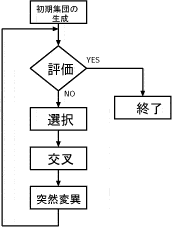
\includegraphics[width=3cm,bb=0 0 172 228]{img/ga.png}
			\caption{遺伝的アルゴリズムの一般的な流れ}
			\label{genetic_algorithm}
		\end{center}
	\end{figure}

	一般的に、遺伝的アルゴリズムは図\ref{genetic_algorithm}のような流れで実装される。

	詳しく説明すると、最初に決められた個体数の染色体がランダムに生成される。染色体はある1つの解を表している。次に、各個体に対して適応度の評価が行われる。適応度はどれだけその個体が優れているかを示したものである。そして、各々の個体に適応度が決定されたら、それを基準に選択/交叉を行い、次世代の遺伝子が生成される。最後に各遺伝子に対して、突然変異という操作を行う。これらの作業を終了すると、新たな世代の個体集団が作られたことになり、この新たな集団に対して、終了条件を満たすまで同じ操作を繰り返し続ける。

	本研究では、選択方法として適応度比例選択とルーレット選択、交叉方法として順序交叉、終了条件を一定時間の経過とした。
	また、使用した適応度関数は、ある個体$i$の解に対応する総移動距離を$d_i$とすると、次式のように表せる。
	\begin{equation*}
		Fitness(i) = \frac{1}{d_i} \times 10^8
	\end{equation*}

\pagebreak
\section{研究結果}
	実験結果を以下の表\ref{result}に示す。
	\begin{table}[htbp]
		\centering
		\begin{tabular}{c||c|c}
			頂点数 & アプローチ1での距離(秒数[s]) & アプローチ2での距離(秒数[s]) \\ \hline
			8 & 847.214(0) & 847.214(0) \\
			9 & 947.214(0) & 947.214(0) \\
			10 & 1047.21(0) & 1047.21(0) \\
			11 & 1147.21(0) & 1147.21(0) \\
			15 & 1907.95(2) & 1907.95(0) \\
			18 & 1976.07(22) & 1976.07(0) \\
			19 & 1986.54(51) & 1986.54(30) \\
			20 & 2038.56(117) & 2038.56(1) \\
			21 & 2079.29(305) & 2079.29(2) \\
			30 & - & 2587.18(71) \\
			50 & - & 3607.60(98) \\
			225 & - & 4121.13(1561) \\
			9847 & - & $6.67068\times10^7$(1817) \\
			
		\end{tabular}
		\caption{実験結果}
		\label{result}
	\end{table}

	アプローチ1はこのまま続けると30頂点で一週間、50頂点だと55823年ほど掛かりそうだったのでそれ以上の頂点数は断念した。アプローチ2に関してはすべて制限時間30分の間で最も良い経路を載せている。\newline

	この結果より、アプローチ1は最適解が求まるが頂点数が増えるに連れ実行時間が大きく増加し、30頂点を超えると1日かけても終わらないようになることが分かった。

	またアプローチ2は、19頂点の場合のように最適解に辿り着くまでに時間がかかったりする事がある。また、アプローチ2の結果だけではそれが最適解である保証がない。しかし頂点数が増加してもアプローチ1と比べるとあまり実行時間は増加せず、しかも最適解が求まることが多いことが分かった。

	この結果より、電子基板に穴を開ける順序を決定する問題などのコストを少しでも削りたいといった問題に関してはアプローチ1のbitを用いた動的計画法を用い、サイズが大きかったり、あまり正確性を求めない問題に対してはアプローチ2の遺伝的アルゴリズムを用いるべきだということがわかった。


	\begin{thebibliography}{4}
			\addcontentsline{toc}{section}{\bibname}
		\item 「遺伝的アルゴリズム - Wikipedia」 2014/2/4最終アクセス \\
			\url{http://ja.wikipedia.org/wiki/遺伝的アルゴリズム}
		\item 「遺伝的アルゴリズム」 2014/2/4最終アクセス \\
			\url{http://www.obitko.com/tutorials/genetic-algorithms/japanese/index.php}
		\item 「村上・泉田研究室 第2章 遺伝的アルゴリズムの処理手順」 2014/2/4最終アクセス \\
			\url{http://ipr20.cs.ehime-u.ac.jp/column/ga/chapter2.html}
		\item 「システムの最適化 - 4. 遺伝的アルゴリズム(GA:Genetic Algorithm) -」 2014/2/4最終アクセス \\
			\url{http://www.sist.ac.jp/~suganuma/kougi/other_lecture/SE/opt/GA/GA.htm}
	\end{thebibliography}

\end{document}
